\documentclass[10pt,sigconf,letterpaper,nonacm]{acmart}
\usepackage{mathtools}

\graphicspath{{../../figures/edgesys2023/}}

\title{Cloud Morphing: A Responsive Model for Distributed Resource Management}

\author{Kenjiro Cho}
\email{kjc@iijlab.net}
\affiliation{\institution{IIJ Research Laboratory}\city{}\country{}}

\author{Jean-François Baffier}
\email{jf@baffier.fr}
\affiliation{\institution{IIJ Research Laboratory}\city{}\country{}}

\begin{document}


\begin{abstract}

    In this paper, we envision future distributed cloud services with
    abundant heterogeneous computing resources,
    and propose to apply dynamic pricing to a responsive model for
    distributed resource management.
    In this model, the pseudo cost of a resource is a function of the
    load, and the required resources for a job are allocated by a simple
    cost minimization algorithm.
    We introduce a convex cost function that enables autonomous
    load-balancing and idle-resource pooling within the cloud, and allows
    stakeholders to loosely control the utilization of each resource by
    manipulating the cost function or the resource weights of micro-jobs.
    We examine different cost tuning methods for adjusting
    utilization, and illustrate their behaviors by simulation.

        % This paper envisions future distributed cloud services with abundant heterogeneous computing resources, and proposes dynamic pricing to a responsive model for distributed resource management. In this model, the pseudo cost of a resource is a function of the load, and the required resources for a job are allocated by a simple cost minimization algorithm. We introduce a convex cost function that enables autonomous load-balancing and idle-resource pooling within the cloud, and allows stakeholders to loosely control the utilization of each resource by  manipulating the cost function or the resource weights of micro-jobs. We examine different cost tuning methods for adjusting utilization, and illustrate their behaviors by simulation.
\end{abstract}

\maketitle

\section{Introduction}

\subsection{Background}

%% cloud and virtualization technologies
Cloud computing was brought about by virtualization technologies,
enabling to build large pools of virtualized computing resources (e.g.,
servers, storage, and network) and dynamically allocate necessary resources
for providing services.
However, cloud computing system itself is still on physical cloud
infrastructure; cloud system operators manually manage
physical servers and network switches to meet the overall demands
so as not to overload certain resources.

The next challenge would be to virtualize cloud infrastructure!
By decoupling infrastructure management from service management,
cloud resources such as servers and networks can be provided with a
pay-as-you-go model.
Then, cloud service operators are liberated from hardware resource management,
as was the case for system administrators by cloud computing.
Moreover, it is not enough to shift responsibility to operators of the
new lower infrastructure layer. We need a new self-managing
infrastructure layer which does not require human operators.

%% Edge computing and micro datacenters
We also consider two recent trends in cloud computing.
One trend is edge computing~\cite{Lopez-2015} and
micro datacenters~\cite{Greenberg-2009}.
Small-scale datacenters with a few racks or even a couple of servers
can be placed at locations closer to the users, to reduce latencies
or to store sensitive data on premise, and make them act as part of
the cloud.
A possible future direction is distributed cloud computing that
utilizes diverse and geographically scattered computing resources.
It will require a new management mechanism to efficiently utilize such
resources.
On the other hand, computing resources will be abundant in the
environment so that it will be no longer necessary to micromanage
computing resources.

%% serverless, micro services
Another trend is microservices~\cite{nadareishvili2016microservice}
and serverless computing~\cite{Shafiei-2022} in which
a cloud service is composed of a collection of loosely-coupled
lightweight services.
Each microservice is ephemeral and short-lived, and can be executed
in a stateless container,
which enables flexible and efficient use of underlying cloud
resources.
The concept has something in common with early packet switching so
that it might open up new possibilities to apply packet switching
techniques to handling microservice jobs.

%% energy saving?
In addition, we should take energy saving into consideration as it is
essential for future clouds~\cite{Mastelic-2015,masanet2020recalibrating}.

\subsection{Cloud Morphing Vision}

{\em Cloud Morphing} is our vision for cloud virtualization in the future.
By dynamically allocating microservices over distributed
heterogeneous resources, a cloud service instance emerges at the best
location and, as the usage pattern changes, the service instance also
transforms the locations of the resources and their connections.

Microservice jobs are assigned to reduce the execution cost that
consists of computing cost, communication cost with the user, access
cost to database, and other factors.
For examples, an interactive task will follow the user when the user
moves, while a data-intensive task will stay close to the data
regardless of the user location.
Edge computing is automatically formed by allocating resources close to
the users.
Moreover, services are inherently fault-tolerant and resilient
against outages or disasters since faulty resources are
automatically evicted from the resource pool.

From the operational perspective, the physical resource management
becomes simpler, since physical nodes can be easily attached to or
detached from the resource pool.
When there is a consistent hotspot, it can be alleviated or solved by
placing new resources close to the hotspot and then attaching them to
the resource pool at a convenient time.

Diverse resources would be owned and managed by different parties.
It requires loose management of resources, as small parties cannot
afford dedicated skilled operators.
The utilization of each resource needs to be easily manipulated,
without affecting the stability of the system.

To realize such systems, it requires various technical advances across
many fields.  Among other things, new autonomous resource management
model is needed for distributed diverse cloud resources,
which is the topic of this short paper.

\subsection{Resource Management}

%% resource allocation problems are NP-hard
%% even harder for distributed heterogeneous resources
Resource allocation in distributed clouds is a non-trivial
optimization problem, and it is even harder when distributed
management is assumed.

%% our idea: use congestion pricing mechanism for automatic load management
To this end, we employ dynamic pricing for decentralized resource
allocation which works as backpressure against congestion.
By design, serious congestion never happens in the system as long as
some resources remain available in the resource pool.

We use pseudo cost for manipulating resource allocation.
Here, pseudo cost is not an actual monetary charge, but it is used to
control resource utilization.

There exist a large body of literature formulating resource allocation
as optimization problems.
In this paper, we use terms and expressions borrowed from optimization
theory. Our goal is, however, not to pursue theoretical optimum
allocations, but to present a practical feedback control model for
distributed resource management.




\section{Resource Management Model}

\subsection{Job Assignment}

\begin{figure}[tb]
  \begin{center}
    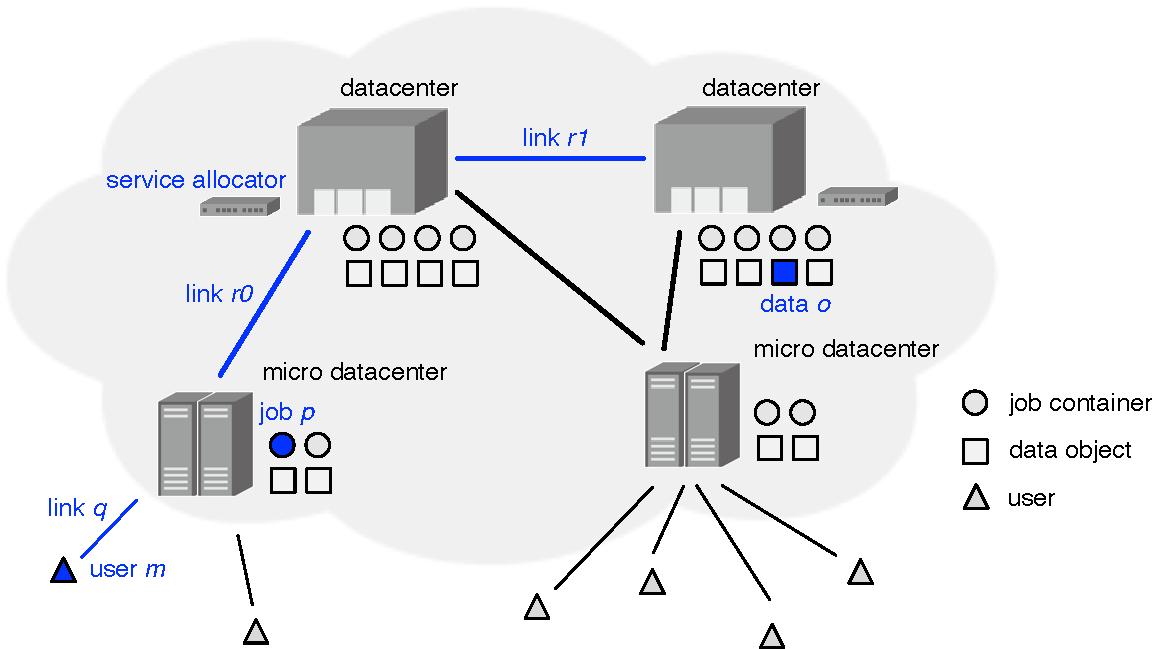
\includegraphics[width=1.0\columnwidth]{system.pdf}
    \vspace{-2.0ex}
    \caption{System model}
    \label{fig:system}
  \end{center}
\end{figure}

A simple system configuration with 2 data centers and 2
micro-datacenters is shown in Figure~\ref{fig:system}.
When a user requests a service to a nearby service allocation server,
the service server instantiates the requested service into a series of
microservice jobs.
The server finds the required resources for each job,
identifies the locations of the user and the required data object,
asks available resources (or their proxies) for the current costs,
and assigns the job to the node with the lowest pseudo cost.
The area for cost inquiry could be within proximity to the path
between the user and the data object.

The load of a resource can be measured in a number of ways.  Most
resources have some form of load report functions built-in.
A load value does not need to be precise, and a rough approximation is
enough for loose resource management.
On the other hand, if each allocation is not small enough both in size
and in duration, the loads may not converge as expected.
That is, microservice is the enabler for this approach.

We use a simple micro job model that defines the required resources
for a micro-job as $J(p, q, r, s)$ where 
$p$ is the number of micro containers, 
$q$ is frontend communication with the user, 
$r$ is backend communication with data objects (e.g., database), and
$s$ is the number of time slots.
%%The unit is one micro-container for $p$, 1Mbps for $q$ and $r$, and 1
%%second for $s$.
For simplicity in the paper, we do not distinguish directions of
communications for $q$ and $r$, and assume only one user and one data
object per job.

A job can be optionally associated with weights for the cost
calculation with $p$, $q$, and $r$: e.g., an interactive job may raise
the weight for the frontend communication to place the job close to
the user.

To instantiate a micro-job requested from a user, the service
server finds the best node to allocate the required resource
for $J$: $p$, $q$ and $r$ for duration $s$.

The pseudo cost $E$ to host job $j$ for a unit time at node $i$ for
user $m$ and data object $o$ is:
\begin{equation*}
	E(j, i)     = H(j,i) + G(j,i,m,o)
\end{equation*}
here, $H(j, i)$ is the computing cost to run $j$ at $i$, and
$G(j, i, m, o)$ is the communication cost to run $j$ at $i$
between $m$ and $o$.
\begin{eqnarray*}
&&  H(j,i)      = p \cdot f(\rho_{i}) \\
&&  G(j,i,m,o)  = q \cdot \smashoperator{\sum_{l \in path(m,i)}} f(\rho_{l}) + r \cdot \smashoperator{\sum_{l \in path(i,o)}} f(\rho_{l})
\end{eqnarray*}
$f(\rho)$ is the cost fuction of a resource load, and $path(m,i)$ is a set
of links from $m$ to $i$ (e.g., the shortest path weighted by cost).

To assign Job $j$, the server simply finds the lowest cost node $i$:
\begin{equation*}
	argmin_{i} \: E(j, i)
\end{equation*}

\subsection{Pseudo Cost Functions}

%% idea: mechanics model instead of optimization

Our model employs a parametric representation of pseudo cost, as a
function of load, and uses it for load control and also as
backpressure against congestion.
Micro-jobs are naturally gravitated to the most cost-efficient
location.

%% model: cost function: congestion pricing combined with idle-resource pooling
The proposed model is based on congestion pricing in which the cost of
a resource dynamically changes according to the load of the resource.
It works as a barrier function for optimization; the capacity
constraint is enforced by a penelizing cost when approaching the full
capacity.

Another key idea is {\em idle-resource pooling} that tries to put resources
into idle state when possible for energy saving.
We proposed a convex cost function that enables idle-resource pooling
by modified congestion pricing.

A pseudo cost function in our model maps the load of a resource
$\rho \in [0, 1]$ to the corresponding cost.
The capacity limit is enforced by the cost function that rapidly grows
as the load approaches $1.0$, which is known as a barrier function in
optimization theory. 

We use two types of pseudo cost functions: one is the monotonic cost
function and the other is the convex cost function.
The monotonic cost function is a simple barrier function that
monotonically grows with load, up to inifinite as $\rho \to 1$.
The convex cost function is also a barrier function but also for
idle-resource pooling.
In this paper, the monotonic form is used for network links as
energy-saving-by-idling is not common for network links.

The standard forms that have the minimum cost of $1.0$ are
shown in Figure~\ref{fig:std_costfunc}. We will show how to manipulate
the cost functions in Sec.~\ref{sec:variation}.

\begin{figure}[tb]
  \begin{center}
    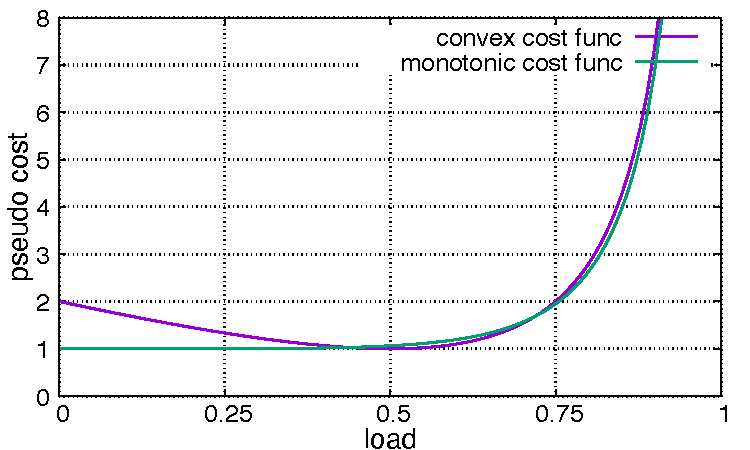
\includegraphics[width=1.0\columnwidth]{costfunc.pdf}
    \vspace{-2.0ex}
    \caption{Standard cost functions}
    \label{fig:std_costfunc}
  \end{center}
\end{figure}

The standard convex cost function is defined as:
\begin{equation*}
	f(\rho) = \frac{(2\rho - 1)^{2}}{1 - \rho} + 1
\end{equation*}
This function has the properties:
$min\: f(\rho) = f(.5) = 1$, and $f(0) = f(.75) = 2$.
The cost grows rapidly when $\rho \ge .75$.
The system automatically tries to keep $\rho \le .75$,
aiming at $\rho = .5$.

The standatd monotonic function is deafined as:
\begin{equation*}
	f(\rho) = \frac{\rho^{4.5}}{1 - \rho} + 1
\end{equation*}
to roughly match the standard convex function in $[.5, .75]$,
the {\em working load range} explained in the next subsection.

Note that the standard forms are defined just for convenience, and
other functions with a similar shape in $[0,1]$ also work for our
purposes.

\subsection{Idle-Resource Pooling in Action}

The behavior of idle-resource pooling by the convex cost function is
illustrated by the following examples in Figure~\ref{fig:4node} and
Figure~\ref{fig:4node-ratio}.

\begin{figure*}[tb]
  \begin{minipage}{1.0\columnwidth}
  \begin{center}
    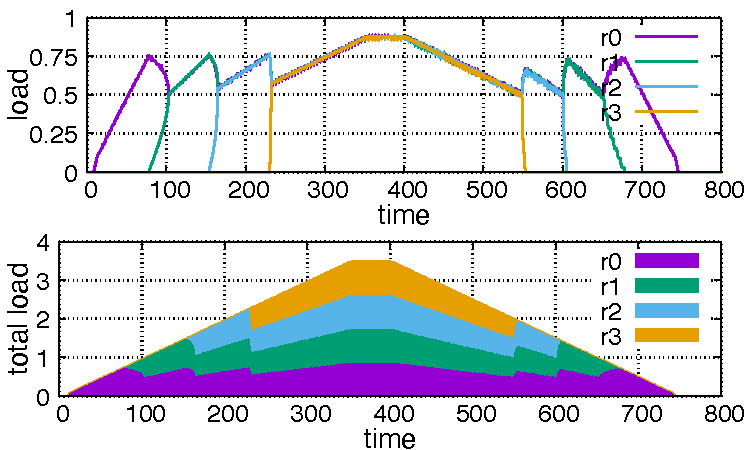
\includegraphics[width=1.0\columnwidth]{4node.pdf}
    \vspace{-2.0ex}
    \caption{load distribution among 4 equivalent cost nodes}
    \label{fig:4node}
  \end{center}
  \end{minipage}
  \hspace{0.8\columnsep}
  \begin{minipage}{1.0\columnwidth}
  \begin{center}
    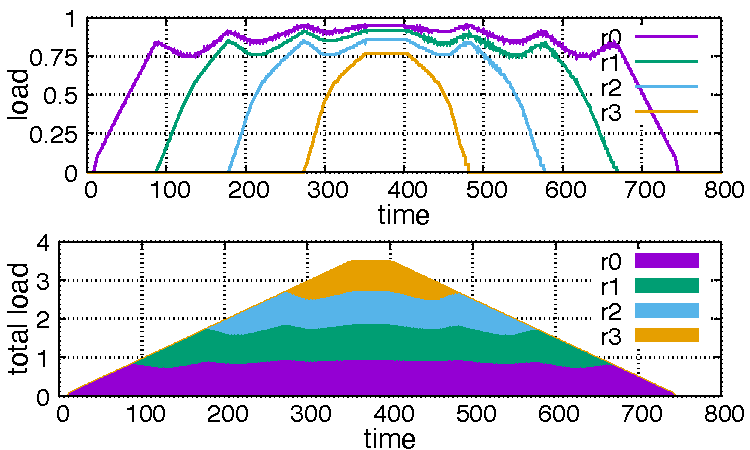
\includegraphics[width=1.0\columnwidth]{4node-ratio.pdf}
    \vspace{-2.0ex}
    \caption{load distribution among 4 proportional cost nodes}
    \label{fig:4node-ratio}
  \end{center}
  \end{minipage}
\end{figure*}

Assume a pool of 4 equivalent resources with the standard convex
cost function.
Also, assume that micro-jobs are continuously assigned to the
system; each micro-job is much smaller than the capacity of a
resource.

The initial system load $\sum \rho$ is $0$, and gradually increased up
to $3.5$ until time 350. After time 400, the system load is gradually
decreasesd back to $0$ until time 750.
Here, load $1.0$ is the capacity of a single resource. 
Initially, all resources in the pool are idle, and their costs are
all $f(0)= 2$.
First, one resource $r_{0}$ is randomly selected for allocation, and its
cost becomes lower: $f(0+) < 2$. As a result, subsequent jobs are
assigned to $r_{0}$, with lowering cost towards $\rho = .5$ and then
rising again until $\rho = .75$ where $f(.75) = 2 = f(0)$.
At this point, another resource $r_{1}$ is selected for allocation.
$r_{1}$ is preferred over $r_{0}$ as its cost becomes lower with new
allocation so that both loads move towards $\rho_{0} = \rho_{1} = .5$,
where both are balanced.
Both loads rise again until $\rho_{r_{0}} = \rho_{r_{1}} = .75$,
where the third resource $r_{2}$ kicks in.
It repeats for $r_{3}$, but no more idle resouce is available
when $\sum \rho$ reaches $3.0$ so that the loads grow beyond $.75$
up to $\sum \rho = 3.5$ with $\rho = .875$ for each.

When the system load decreases, the process is reversed.
After reaching $\rho = .5$ for all,
one resource with the lowest load $\rho < .5$ becomes more expensive
than the others.
This one is less preferred for subsequent assignments, and quickly
loses the load until it becomes idle again, while the other 3 keep
$\rho$ in $[.5, .75]$. It repeats for the remaining ones.

It is easy to see how the number of active resources changes when
there are more resources.
When the number of active resources is increasing, the load of each
active resource stay at around $\rho = .75$.
On the other hand, when the number of active resources is decreasing,
the load of each active resource stay at around $\rho = .5$.
In short, when all resources are equal, the system tries to maintain
the load of active resources in the {\em working load range}
$[.5, .75]$, while keeping idle resources as much as possible.

When resources are not equal, the behavior becomes more complex, but
the underlying mechanisms are the same.
Let's take a look at a case of 4 resources with the cost ratio $1:2:4:8$,
that is $8 f_{r_{0}} = 4 f_{r_{1}} = 2 f_{r_{2}} = f_{r_{3}}$ in
Figure~\ref{fig:4node-ratio}.
To activate $r_{1}$, the load of $r_{0}$ goes up to $.84$ to satisfy:
$f_{r_{1}}(0) = 4 = f_{r_{0}}(.84)$.
When $r_{1}$ is moving towards idle after time 550, the load
of $r_{0}$ is $.75$ to satisfy: $f_{r_{1}}(.5) = 2 = f_{r_{0}}(.75)$

For unequal resources in general, the required load to trigger new
resource allocation would be higher than $\rho = .75$ for the already
active ones to match the cost $f(0)$ for the new one, but the load
will not go much further as the slope of the cost function is steep.
Similarly, when the most expensive one among active resources becomes
idle, the load of the remaining ones stay at the matching cost at
$f(.5)$ for the deactivating one.

When the load of a resource fluctuates too rapidly,
a smoothing filter such as an exponetially weighted moving average
can be used to stabilize the behavior.

Note that our goal is not to achieve the theoretical optimum but to
enable loose automatic distributed load balancing.

\subsection{Manipulating the Cost Function}
\label{sec:variation}

The utilization of a resource can be manipulated by modifying the cost
function of the resource as shown in Figure~\ref{fig:costfunc3}.

One can {\bf lower or raise the utilization} of a resource by raising or
lowering the cost.
To make the cost $n$ times more expensive, $f'(\rho) = n f(\rho)$.
For minor adjustment, one can use an additive form,
$f'(\rho) = f(\rho) + \Delta$.

The {\bf idle-state can be made stickier} by raising the cost at $\rho = 0$:
e.g., to raise the cost at $\rho = 0$ by a factor of $n$,
$f'(\rho) = n (2\rho - 1)^{2}/(1 - \rho^{n}) + 1$.

A {\bf premium service} can be realized by lowering the target load so
that premium jobs are always assigned to lightly loaded resources, 
$f'(\rho) = f(\rho + \Delta)$.
Similary, an {\bf economy service} can be made by raising the target
load.

\begin{figure}[tb]
  \begin{center}
    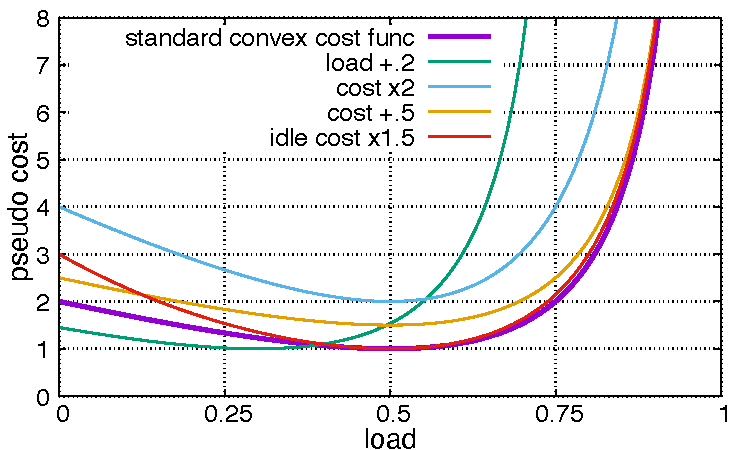
\includegraphics[width=1.0\columnwidth]{costfunc3.pdf}
    \vspace{-2.0ex}
    \caption{Manipulating convex cost functions}
    \label{fig:costfunc3}
  \end{center}
\end{figure}


\begin{figure}[tb]
  \begin{center}
    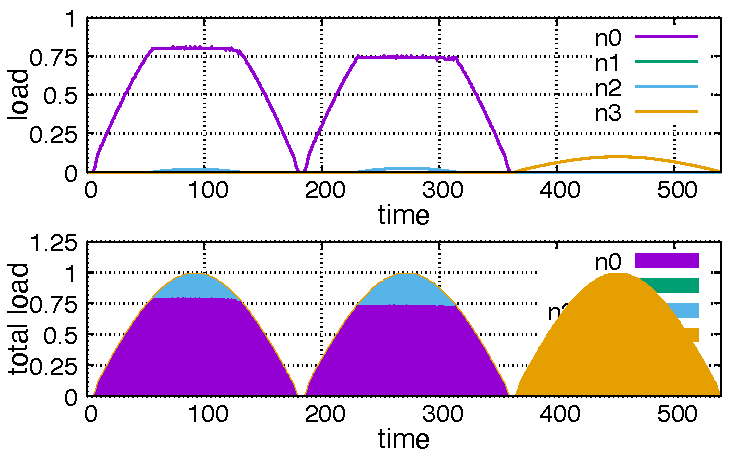
\includegraphics[width=1.0\columnwidth]{lowering.pdf}
    \vspace{-2.0ex}
    \caption{Data intensive and interactive jobs}
    \label{fig:lowering}
  \end{center}
\end{figure}

In Figure~\ref{fig:lowering}, 3 waves of jobs are generated between
user~0 (at node~0) and object~0 (at node~3).
The load of n2 and n3 are drawn as $x10$ to compare the quantity of n0
and n1 because of the difference in their capacity.
The first wave contains only data intensive jobs, and all jobs are
assigned to the node that has the object (n3).
The second and third waves contain only interactive jobs, and most of
the jobs are assigned to the node closest to the user (n0) but some
overflowing jobs are assigned to n2.
In the third wave, the cost function of n0 is manipulated to reduce
the load by multiplying the cost function by 1.5.a


\section{Simulation Results}


We have developed a simple simulation tool to evaluate the model
that is publicly available from (URL removed for blind-review).
We omit the details of the simulation settings in this paper but all
the settings are described in the simulation tool.

%%\subsection{Simulation settings}

%%The simulation setting is shown in Figure~\ref{fig:topology-simple}.
%%\begin{itemize}
%%  \item		job: mean duration:4sec, mean 1 unit,
%%        frontend 1, backend 2 for data intensive job,
%%        frontend 2, backend 1 for interactive job,
%%  \item		node: capacity 100 for MDC, 1000 for DC
%%  \item		link: capacity 200 for MDC-DC, 1000 for DC-DC
%%\end{itemize}
%%
%%\begin{figure}[tb]
%%  \begin{center}
%%    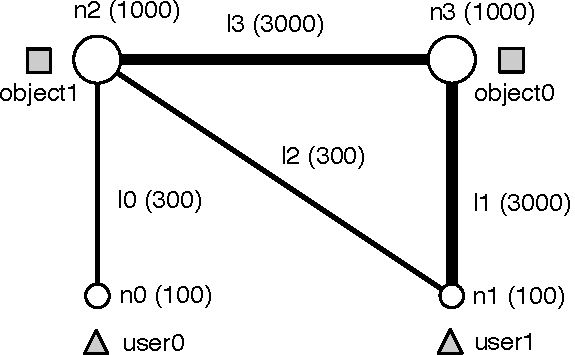
\includegraphics[width=7.5cm,clip]{topology-simple.pdf}
%%    \vspace{-2.0ex}
%%    \caption{simple simulation topology}
%%    \Description{Simulation topology with 2 datacenters and 2 micro datacenters.}
%%    \label{fig:topology-simple}
%%  \end{center}
%%\end{figure}
%%
%%Simulation scenarios:
%%\begin{enumerate}
%%  \item	{\bf node only:} 4 nodes without randomization to show how the
%%        cost function works
%%  \item	{\bf link only:} 4 links without randomization to show
%%        different costs affects
%%  \item	{\bf monotonic function:} same as above but use monotonic cost
%%        function.
%%  \item	{\bf randomize:} 4 nodes and 4 links with randomization
%%  \item {\bf comparison:} compared with, no idle-resource pooling
%%  \item	{\bf surge:} same as above but with a request surge at one location
%%  \item	{\bf edge computing:} 2 nodes (big and small) and 1 link, the
%%    users are closer to the small node. 2 types jobs (interactive,
%%    data intensive).  show interactive jobs are on the small node,
%%    data intensive jobs are on the big node.
%%  \item {\bf premium service:} 4 nodes with 3 standard and 1 premium services.
%%  \item	{\bf complex?:} realistic scenario
%%\end{enumerate}

\subsection{Basic Behaviors}

\begin{figure}[tb]
  \begin{center}
    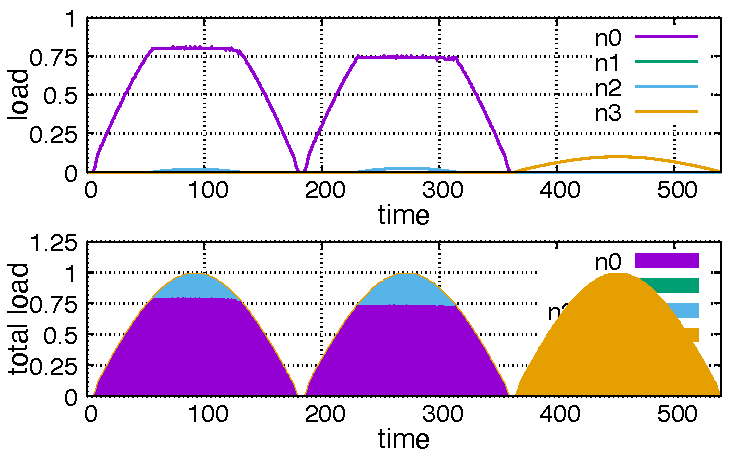
\includegraphics[width=1.0\columnwidth]{lowering.pdf}
    \vspace{-2.0ex}
    \caption{Cost manipulations: shifting the load +.2,
      +.4 and raising the weight for data access}
    \smallskip
    \raggedright
    \small
    Note that the capacity of DCs is 10 times larger than that of MDCs
    so that DC's load looks much smaller for the same volume of jobs.
    In the normalizede total load (bottom), the volume is normalized
    to the capacity of MDC to show the total volume of jobs:
    $\sum \tilde{\rho}$, \:$\tilde{\rho} = \rho \cdot C/C_{MDC}$.
    \Description{Simulation results to illustrate the effects of cost manipulations.}
    \label{fig:lowering}
  \end{center}
\end{figure}

The effects of manipulating the cost function and the resource weight
for a job is illustrated in Figure~\ref{fig:lowering}.
Here, a series of interactive jobs of the same type are generated in
4 waves between a user at MDC0 and an object at DC3 in
Figure~\ref{fig:system}.
In the first wave,  most of the jobs are assigned to the node closest
to the user (MDC0) but some overflowing jobs are assigned to DC2.
The peak load of MDC0 is .80 in the first wave.
In the second and the third waves, the cost function of MDC0 is
manipulated to reduce the load by shifting the load by $.2$ and $.4$
respectively. As a result, the peak load of MDC0 is
reduced from $.8$ to $.6$ in the second wave, and then, to $.4$ in the
third wave.
In the fourth wave, the weight for the backend communication is
increased, and all jobs are assigned to the node that has the object
(DC3).

\subsection{Mixed Behaviors}

A more complex scenario is shown in Figure~\ref{fig:mixed}.
Again, the topology in Figure~\ref{fig:system} is used, and
random fluctuation is added to the interval and duration of jobs.
A series of jobs are generated
between user0 at MDC0 and an object at DC3, and
between user1 at MDC1 and an object at DC2.
Both have the ratio of $1:2$ for interactive vs. data-intensive jobs.
To observe offloading behaviors, user1's jobs are increased by a
factor of 2 in the third wave (time 360-540), and by a factor of 10 in
the fourth wave (time 540-720). 
Before time 360, interactive jobs are assigned closer to the user,
and data intensive jobs are assigned closer to the data.
In the third wave, MDC1 reaches the upper limit and overflowing jobs are
assigned to DC2.
In the fourth wave, the link MDC1-DC2 reaches the upper limit so that
overflowing jobs are assigned to DC3.
(To absorb the surge in the fourth wave in this scenario, enough
capacity is provided to the link MDC1-DC3.)
This scenario illustrates the responsive behavior of the system,
and how jobs for micro datacenters can be offloaded to upstream data
centers.

\begin{figure}[tb]
  \begin{center}
    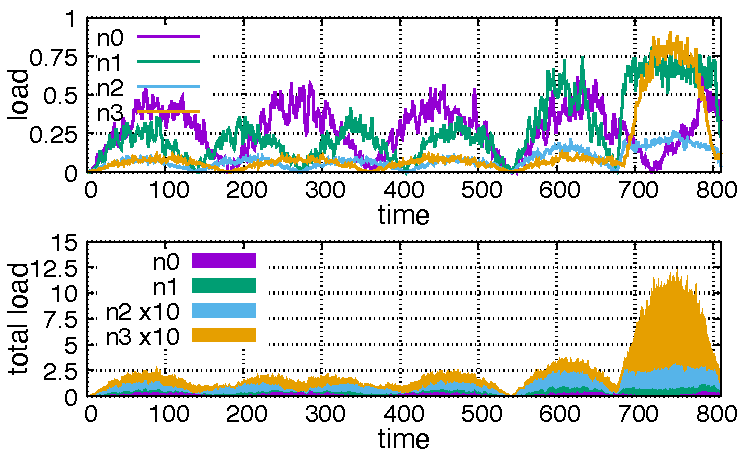
\includegraphics[width=1.0\columnwidth]{simu2.pdf}
    \vspace{-2.0ex}
    \caption{Mixed load with 2 DCs and 2 MDCs}
    \Description{Simulation results with mixed scenario.}
    \label{fig:mixed}
  \end{center}
\end{figure}

% \begin{figure}[tb]
%   \begin{center}
%     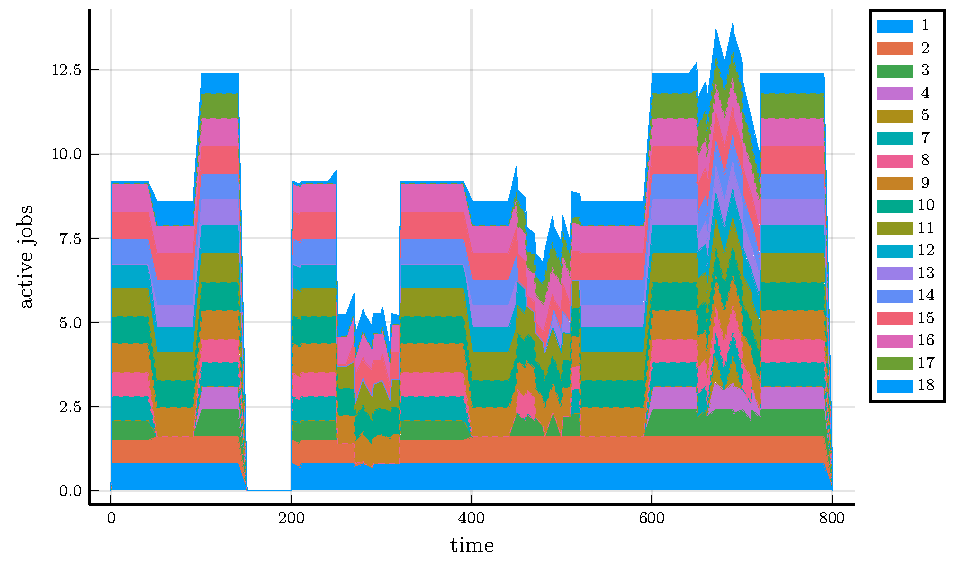
\includegraphics[width=1.0\columnwidth]{complex-convex-monotonic.pdf}
%     \vspace{-2.0ex}
%     \caption{Complex scenario with convex nodes and monotonic links}
%     \label{fig:complex}
%   \end{center}
% \end{figure}

% \begin{figure}[tb]
%   \begin{center}
%     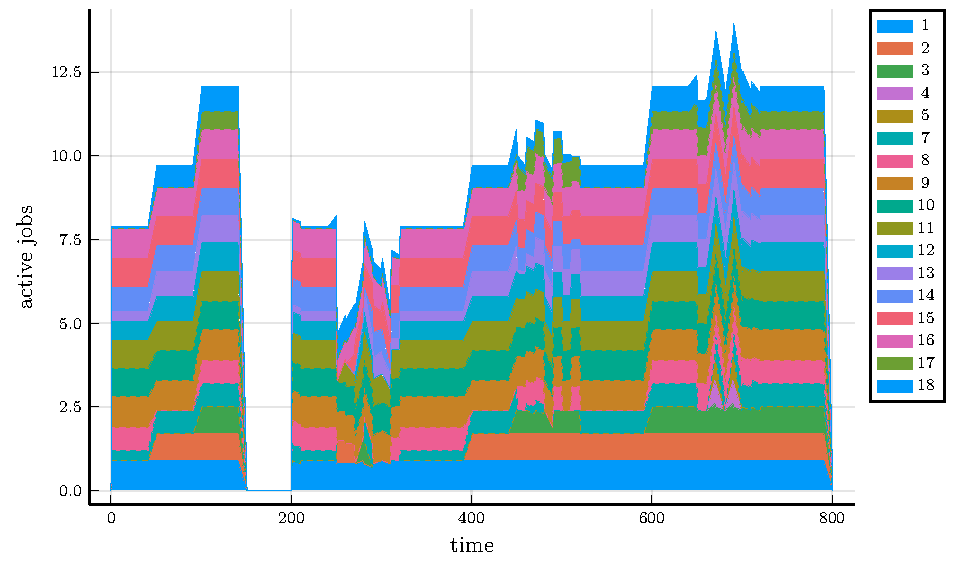
\includegraphics[width=1.0\columnwidth]{complex-full-convex.pdf}
%     \vspace{-2.0ex}
%     \caption{Complex scenario with convex nodes and monotonic links}
%     \label{fig:complex-convex}
%   \end{center}
% \end{figure}

% \begin{figure}[tb]
%   \begin{center}
%     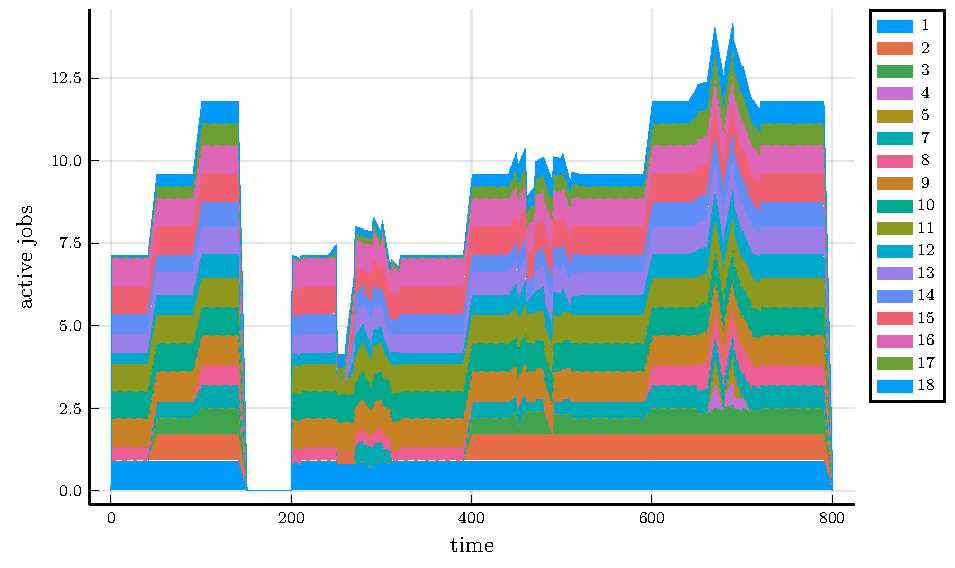
\includegraphics[width=1.0\columnwidth]{complex-full-monotonic.pdf}
%     \vspace{-2.0ex}
%     \caption{Complex scenario with convex nodes and monotonic links}
%     \label{fig:complex-monotonic}
%   \end{center}
% \end{figure}

\begin{figure}[tb]
  \centering
  \begin{subfigure}{\columnwidth}
      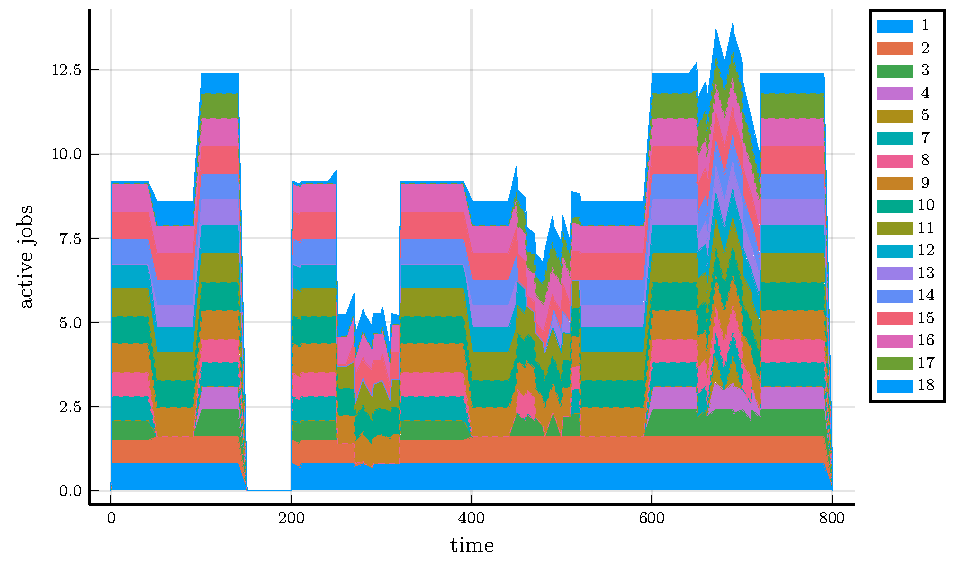
\includegraphics[width=\textwidth]{complex-convex-monotonic.pdf}
      \caption{Convex nodes and monotonic links}
      \label{fig:first}
  \end{subfigure}

  \begin{subfigure}{\columnwidth}
      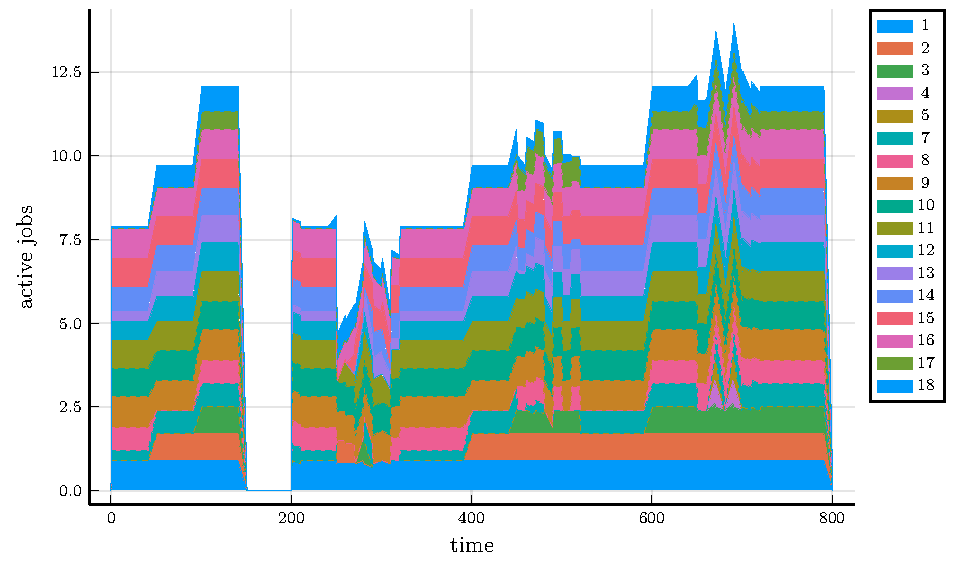
\includegraphics[width=\textwidth]{complex-full-convex.pdf}
      \caption{Convex nodes and links}
      \label{fig:second}
  \end{subfigure}

  \begin{subfigure}{\columnwidth}
      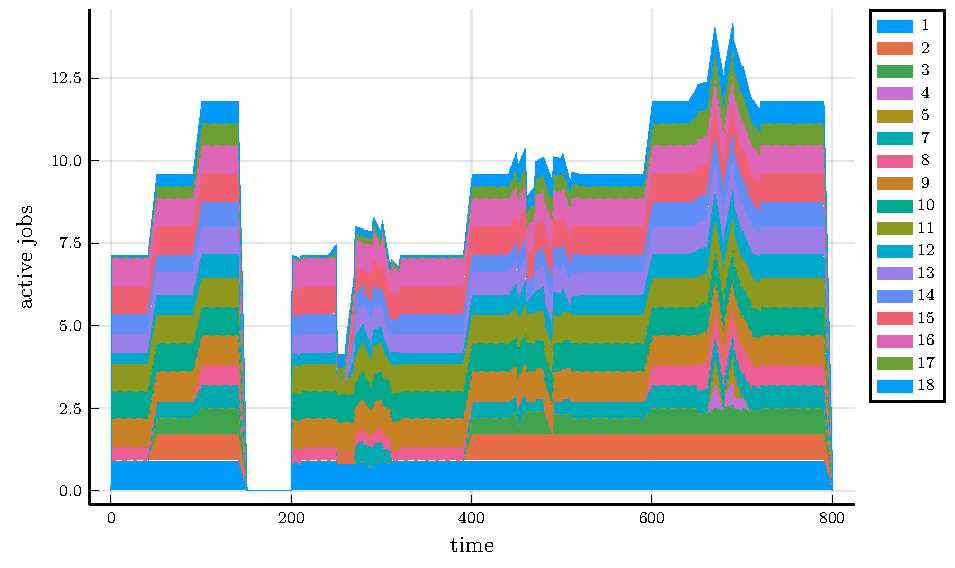
\includegraphics[width=\textwidth]{complex-full-monotonic.pdf}
      \caption{Monotonic nodes and links}
      \label{fig:third}
  \end{subfigure}

  \caption{Comparison of convex and monotonic resources in a complex scenario}

  \label{fig:figures}
  \end{figure}

The last scenario shows a more complex case with 18 DCs: 2 core-DCs, 8
local-DCs and 8 leaf-DCs connected by a FAT-tree.  Each leaf is
connected to one local-DC, but a local-DC is connected to 2 core-DCs
and 2 other local-DCs, or just to 2 other local-DCs.
Jobs are generated from all leaf-DCs and local-DCs.

The load of leaf-DCs and local-DCs are mostly around the target load
$.75$.
This simulation result illustrates
quick responses to changing load,
yet converging to stable states once the load is settled,
and offloading excess jobs to upstream data centers.



\section{Related Work}

Resource allocation for edge computing and micro data centers has
a rich collection of work; most approaches are based on some form of
optimization and many employ auction models.
The topics are ranging from VM auctions in
IaaS~\cite{Zhang2017-VMauction,Zaman-2013},
load balancing within a data center~\cite{Rikhtegar2021BiTEAD,Chen-SOCC-2014},
to
distributed resource management~\cite{Alicherry-INFOCOM2012} for microservices~\cite{Suresh-SOA-SOCC2017}.
Xu {\em et al.}~\cite{Xu2017-zenith} proposed an auction model for
the edge computing infrastructure layer that is similar to
our system model in separating the infrastructure layer.

Congestion pricing and smart data pricing for networking have been
extensively studied~\cite{Sen-2013}.
%Early work includes congestion pricing by
%Murphy {\em et al.}~\cite{MURPHY19941053},
%and auction-based resource allocation by
%MacKie-Mason {\em et al.}~\cite{pricing-internet-1994}, both in 1994.
Kelly {\em et al.}~\cite{Kelly-1998} framed congestion pricing in an
optimization framework for fair allocation, which inspired a large
number of the following
work~\cite{Sen-2013,gibbens1999resource}.
Congestion pricing are also applied to cloud
computing~\cite{Wang-hotcloud2010,Kilcioglu-SIGMETRICS2015,Song-INFOCOM2017}.

Exponential cost growth as a function of load is well known in packet
switching networks (e.g., M/M/1 queue and CSMA/CD Ethernet).
The idea to use such cost functions for resource management
was in \cite{MURPHY19941053} where
Murphy {\em et al.} used a cost function for distributed bandwidth
allocation in ATM networks in 1994.
Their cost function is a barrier function for utility optimization
and their simple cost minimizing allocation algorithm is also somewhat
similar to our allocation model.

A system model similar to ours is found in~\cite{Wagner-2012} where
Wagner {\em et al.} used congestion pricing for resilient job
allocation in a distributed military cloud.  They used a
game-theoretic resource allocation method based on Nash Bargaining,
and developed a Hadoop-based prototype system.

We were inspired by the concept of micro cloud services to apply packet
switching techniques to distributed heterogeneous clouds, and have
revisited congestion pricing.
To the best of our knowledge, our work is unique in using a convex
cost function for idle-resource pooling.

%%data migration\cite{Pu2015-geodistdata}.
%%distributed data store\cite{Shima2012,Tahoe-2008}.




\section{Summary and Future Work}

%% summary and future work

In this paper, we have presented the cloud morphing vision for
future distributed cloud services,
proposed a resource allocation model based on cost functions,
and presented how the idle-resource pooling works.
We are planning to refine the proposed model and develop a working
prototype system.
For the model refinement,
the current model is simplistic so that we will add bidirectional
communication costs,
multiple users per job, interactions among jobs, and other features.
We did not consider dependency among microservice jobs, but it would be
necessary to investigate the impact of the interplay of microservice
jobs ~\cite{Suresh-SOA-SOCC2017}.
For the prototype development,
we need realistic future microservice workload models.
Also, it is necessary to develop mechanisms and protocols for
discovering available resources~\cite{Albrecht2008} and exchanging
cost information.
A path selection mechanism is also needed when assigning a job,
probably using a source routing mechanism.
There exists a rich area for further research:
one topic is {\bf auto-tuning of the cost functions}.
It may not be straightforward to obtain expected results by tuning the
convex cost function due to the interactions between load-balancing
and idle-resource pooling.
It would be interesting to apply reinforcement learning to cost
tuning.
Another topic is {\bf hierarchical configurations}.
A hierarchical system model would be preferred for scalability
and for management purposes.
For example, a distributed datacenter model can consist of
the inter-DC layer with DC-level resources and the intra-DC layer
with rack-level resources.
The proposed system was originally designed mainly for a single
administrative domain.
The hierarchical model, however, naturally extends to
an {\bf inter-cloud model} in which different cloud systems are
federated.
The mechanism of the idle-resource pooling allows utilizing external
clouds only when needed.
Further, it would be possible to {\bf crowdsource the resource supply}
at the edge. 
Then, we need a monetary charging, authentication and authorization
mechanisms to add externally provided resources to the resource pool.
The location of data is critical for the pseudo cost so that
{\bf data placement} would play an important role for cloud morphing. 
A possible approach is to migrate data at a coarser timescale, based
on usage history.
Another possibility is to design a new distributed storage system
suitable for the cloud morphing model in which (cached) data can be
easily moved.
The idle-resource pooling is not used for network links in this paper, but
it is possible to use it for dynamically making {\bf Layer 2 paths}
(e.g., lightpath switching over WDM networks).
We believe that future distributed heterogeneous clouds need a new
paradigm for resource management, and hope this work will stimulate
other research in the field.


\bibliographystyle{ACM-Reference-Format}
\bibliography{cloudmorphing}

\end{document}
